\documentclass[final]{beamer} 
\usepackage[orientation=portrait,size=a1,scale=1.09]{beamerposter} 

\usepackage[portuguese]{babel}
\usepackage[utf8]{inputenc}

% para poder usar imagens eps e psfrag

%\usepackage{epstopdf} 
%\usepackage{epsfig}
\usepackage{graphicx}
\newcommand{\tdots}{\,.\,.\,} % in place of \ldots
\usepackage{mathtools}
\usepackage{tikz}
\usepackage{tikz-qtree}
\usetikzlibrary{matrix,backgrounds, decorations.pathreplacing, automata, arrows}
\usepackage{subfig}
\usepackage{tcolorbox}

\usepackage[noend]{algpseudocode}
\usepackage{algorithm}
\floatname{algorithm}{Algoritmo}
\renewcommand{\listalgorithmname}{Lista de Algoritmos}
\renewcommand{\algorithmicrequire}{\textbf{Requer:}}
\renewcommand{\algorithmicensure}{\textbf{Garante:}}
\renewcommand{\algorithmicend}{\textbf{Fim}}
\renewcommand{\algorithmicif}{\textbf{Se}}
\renewcommand{\algorithmicthen}{\textbf{então}}
\renewcommand{\algorithmicelse}{\textbf{senão}}
\renewcommand{\algorithmicfor}{\textbf{Para}}
\renewcommand{\algorithmicdo}{\textbf{faça}}
\renewcommand{\algorithmicwhile}{\textbf{Enquanto}}
\renewcommand{\algorithmicfunction}{\textbf{Algoritmo}}
\renewcommand{\algorithmicreturn}{\textbf{Devolva}}


\newcommand{\E}{\Sigma}
\newcommand{\cS}{\mathcal{S}}
\newcommand{\Oh}{\mathcal{O}}
\renewcommand{\emph}[1]{\textbf{#1}}


\newcommand{\PP}{\mbox{P}}
\newcommand{\NP}{\mathit{NP}}
\newcommand{\PL}{\mathit{PL}}
\newcommand{\PLI}{\mathit{PLI}}
\newcommand{\OPT}{\mbox{OPT}}

\newtheorem{teo}{Teorema}[section]  % numerado por section
\newtheorem{lema}[teo]{Lema}        % numerado como teo
\newtheorem{cor}[teo]{Corolário}    % numerado como teo
\newtheorem{fato}[teo]{Fato}        % numerado como teo
\newtheorem{mdef}[teo]{Definição}   % numerado como teo

\newcommand{\emptystring}{\varepsilon}

%cardinalidade
\newcommand{\card}[1]
{\left|#1\right|}

\let\:=\colon
\let\epsilon=\varepsilon

%\def\({\left(}
%\def\){\right)}
\def\<{\langle}
\def\>{\rangle}

% valor (e.g., de uma solução)
\newcommand{\Val}[1]
{\mathrm{val}\(#1\)}


% cores utilizadas para os algoritmos
\usepackage{framed}
\definecolor{azul}{rgb}{0.76471,0.81176,0.91373}  % c3cfe9 -> 195,207,233 -> 0.76471   0.81176   0.91373
\definecolor{lilas}{rgb}{0.83529,0.80784,0.89804} % d5cee5 -> 213,206,229 -> 0.83529   0.80784   0.89804
\definecolor{ops}{rgb}{0.9,0.9,0.9} % d5cee5 -> 213,206,229 -> 0.83529   0.80784   0.89804

\urlstyle{same}

%==The poster style============================================================
\usetheme{poster-exemplo}            % our poster style
%--set colors for blocks (without frame)---------------------------------------
  \setbeamercolor{block title}{fg=dblue,bg=white}
  \setbeamercolor{block body}{fg=black,bg=white}
%--set colors for alerted blocks (with frame)----------------------------------
%--textcolor = fg, backgroundcolor = bg, dblue is the jacobs blue
  \setbeamercolor{block alerted title}{fg=dblue,bg=gray!50}%frame color
  \setbeamercolor{block alerted body}{fg=black,bg=gray!20}%body color
%
%==Title, date and authors of the poster=======================================
\title{Algoritmos de Aproximação para Problemas de Clustering}
\author{João Guilherme Alves Santos \hspace{100pt} Orientadora: Cristina Gomes Fernandes}
\institute{\vspace{10pt}{\large Departamento de Ciência da Computação,
Instituto de Matemática e Estatística, Universidade de São Paulo}}
%\date{\today}


%==============================================================================
%==the poster content==========================================================
%==============================================================================
\begin{document}
%--the poster is one beamer frame, so we have to start with:
\begin{frame}[t]
%--to seperate the poster in columns we can use the columns environment
\begin{columns}[t] % the [t] options aligns the columns content at the top
%--the left column-------------------------------------------------------------
%\begin{column}{0.28\paperwidth}% the right size for a 3-column layout
\begin{column}{.9\paperwidth}% the right size for a 3-column layout
	\begin{alertblock}{Introdução}
    Problemas de clustering têm por objetivo agrupar objetos de maneira que objetos no mesmo cluster apresentam mais semelhanças quando comparados a objetos em clusters diferentes. Resumidamente, os problemas que estudamos buscam encontrar uma maneira menos custosa de posicionar instalações para melhor atender um conjunto de clientes. Os clientes estarão em um mesmo cluster se a instalação mais próxima a eles for a mesma. Neste trabalho estudamos vários algoritmos de aproximação e resultados de inaproximabilidade para três problemas de clustering $\NP$-difíceis: $k$-medianas, $k$-centros e localização de instalações. Esses problemas são muito conhecidos e importantes nas áreas de pesquisa operacional e otimização combinatória.
    \end{alertblock}

    \end{column}
\end{columns}
\vspace{1.2cm}

\begin{columns}[t]

  \begin{column}{0.47\paperwidth}

    \begin{alertblock}{$k$-Centros métrico}
      Dado um grafo completo $G$, um inteiro $k$ e uma métrica $c : V(G)\times V(G) \rightarrow \mathbb{R}_+$, encontrar $S \subseteq V(G)$ com $|S| = k$ que minimize $\max_{j \in V(G)} c(j,S)$ em que $c(j,S) \coloneqq \min_{i \in S} c_{ij}$.
    \end{alertblock}
    \begin{block}{Aproximação para o $k$-centros métrico}
      O seguinte algoritmo guloso de González\ [1] é uma 2-aproximação para o $k$-centros métrico: escolha uma cidade qualquer para construir a primeira instalação e, iterativamente, escolha a cidade mais distante das instalações já escolhidas.
      
      % Para o problema dos $k$-centros métrico, escolhemos descrever aqui uma 2-aproximação gulosa, desenvolvida por González [1]. O algoritmo é simples: começamos escolhendo arbitrariamente uma cidade para construir uma instalação e vamos, iterativamente, escolhendo a cidade mais distante do conjunto das instalações já escolhidas.
          \definecolor{shadecolor}{named}{azul}
          \begin{shaded}
            \vspace{-.65cm}
            \begin{algorithm}[H]
              \caption{Guloso-González$(G,c,k)$}
              \begin{algorithmic}[1]
                \State Escolha arbitrariamente $u \in V(G)$.
                \State $S \gets \{u\}$
                \While{$|S| < k$}
                \State $v \gets \arg\max_{j \in V} c(j,S)$
                \State $S \gets S \cup \{v\}$
                \EndWhile
                \State\Return $S$
              \end{algorithmic}
            \end{algorithm}
            \vspace{-.65cm}
          \end{shaded}
        


      \begin{columns}
        \begin{column}{0.23\paperwidth}
        
            \begin{tcolorbox}
              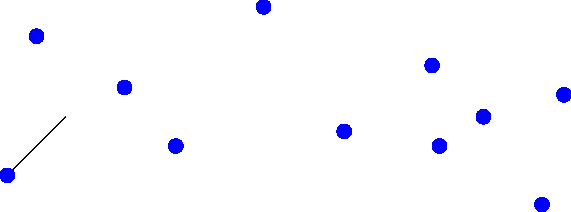
\includegraphics[scale=1.2]{imgs/local-search1.pdf}
            \end{tcolorbox}
            
            \begin{tcolorbox}
              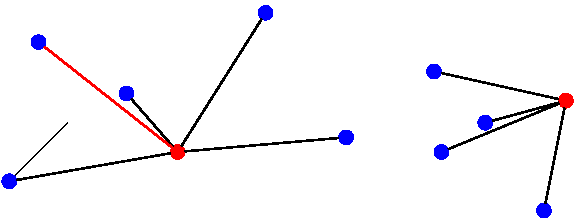
\includegraphics[scale=1.2]{imgs/cent3.pdf}
            \end{tcolorbox}
         \end{column}

         \begin{column}{0.23\paperwidth}
          \begin{tcolorbox}
            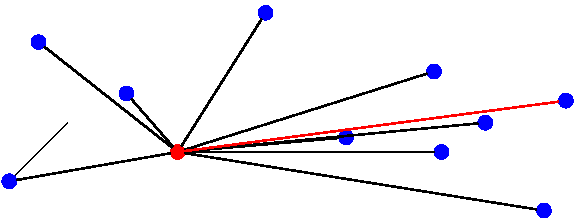
\includegraphics[scale=1.2]{imgs/cent2.pdf}
          \end{tcolorbox}

          \begin{tcolorbox}
            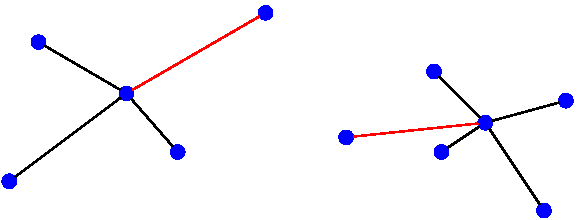
\includegraphics[scale=1.2]{imgs/cent4.pdf}
          \end{tcolorbox}
        \end{column}
      \end{columns}

% Considere uma instância métrica simples com catorze vértices divididos em dois grupos de sete vértices e $k = 2$. As arestas desse grafo têm custo 1, 2 ou 3. Quando induzido pelas arestas de custo 1, cada um dos dois grupos forma uma estrela e, quando adicionadas as arestas de custo~2, cada grupo vira um grafo completo. As arestas de custo 3 ligam os dois grupos. A solução ótima tem custo 1 e consiste em escolher os dois centros das estrelas. A solução abaixo poderia ser sido produzida pelo algoritmo Guloso-González e tem custo 2.
\end{block}

\begin{alertblock}{$k$-Medianas métrico}
  Dado um grafo completo $G$, um inteiro $k$ e uma métrica $c : V(G)\times V(G) \rightarrow \mathbb{R}_+$, encontrar $S \subseteq V(G)$ com $|S| = k$ que minimize $\scalebox{2}{$\sum$}_{j \in V(G)}\, c(j,S)$ em que $c(j,S) \coloneqq \min_{i \in S} c_{ij}$.
\end{alertblock}

\begin{block}{Aproximação para o $k$-medianas métrico}
    Para esse problema descreveremos uma 5-aproximação que usa busca local, de Arya et al.\ [2]. O algoritmo começa com uma solução viável qualquer e vai trocando uma instalação aberta por uma fechada caso a troca melhore o custo, até não haver troca que melhore a solução.
    \definecolor{shadecolor}{named}{azul}
    \begin{shaded}
      \vspace{-.65cm}
      \begin{algorithm}[H]
        \caption{BuscaLocal-AGKMMP$(G = (V,E),c,k)$}
              \begin{algorithmic}[1]
            \State Seja $S$ um conjunto arbitrário com $k$ elementos de $V$.
            \While{existir $u,v \in F$ tal que $u\in S$ e custo$(S - u + v) < $ custo$(S)$}
            \State $S \gets S - u + v$
            \EndWhile
            \State\Return $S$
          \end{algorithmic}
      \end{algorithm}
      \vspace{-.65cm}
      \end{shaded}


      \begin{columns}
        \begin{column}{0.23\paperwidth}
        
            \begin{tcolorbox}
              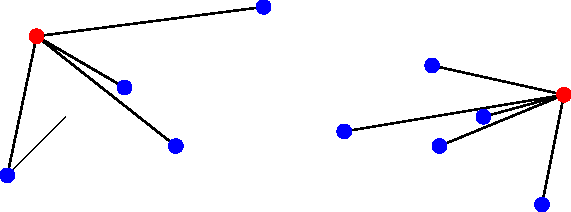
\includegraphics[scale=1.2]{imgs/local-search2.pdf}
            \end{tcolorbox}
            
            \begin{tcolorbox}
              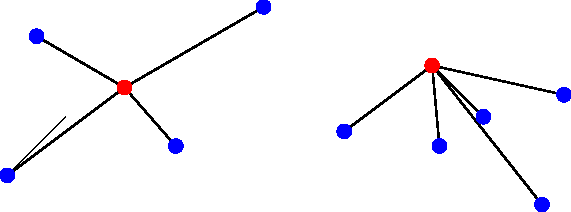
\includegraphics[scale=1.2]{imgs/local-search4.pdf}
            \end{tcolorbox}
         \end{column}

         \begin{column}{0.23\paperwidth}
          \begin{tcolorbox}
            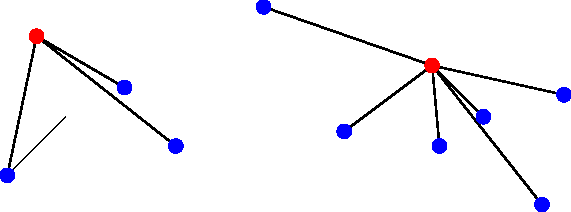
\includegraphics[scale=1.2]{imgs/local-search3.pdf}
          \end{tcolorbox}

          \begin{tcolorbox}
            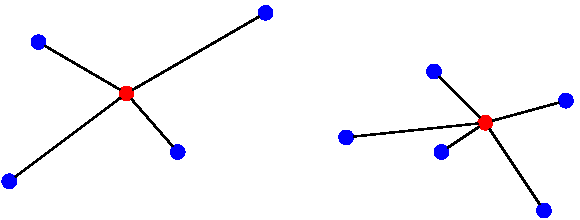
\includegraphics[scale=1.2]{imgs/local-search5.pdf}
          \end{tcolorbox}
        \end{column}
      \end{columns}
      \vspace{0.5cm}
      Esse algoritmo pode ser parametrizado em um número $p$ e, no lugar de trocar apenas um par de instalações, podemos trocar um par de conjuntos de instalações com tamanho no máximo $p$. Essa parametrização resulta em uma $(3 + \frac{2}{p}$)-aproximação para o problema das $k$-medianas métrico que por muito tempo se manteve como o melhor algoritmo de aproximação para esse problema.

        % \fbox{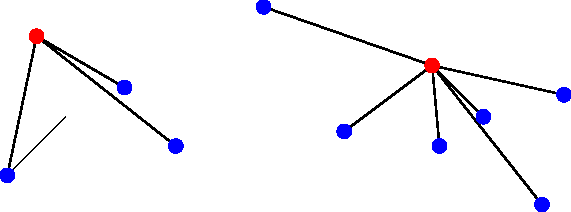
\includegraphics[scale=1]{imgs/local-search3.pdf}} \hspace{2cm}
        % \fbox{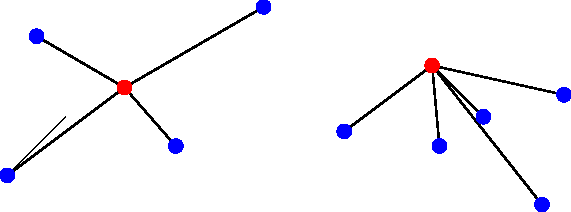
\includegraphics[scale=1]{imgs/local-search4.pdf}} \hspace{2cm}
        % \fbox{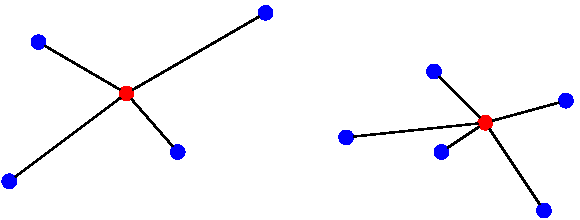
\includegraphics[scale=1]{imgs/local-search5.pdf}} \hspace{2cm}
\end{block}
\begin{block}{Referências}
      
      
  [1]T. F. Gonzalez. Clustering to minimize the maximum intercluster distance.
  Theoretical Computer Science, 38:293–306, 1985.
  
  [2]V. Arya, N. Garg, R. Khandekar, K. Munagala, and V. Pandit. Local search heuristics for $k$-median and facility location problems. SIAM
  Journal on Computing, 33, 2003.
  
  [3]K. Jain and V. Vazirani. Approximation algorithms for metric facility location and $k$-median problems using the primal-dual schema and lagrangian
  relaxation. J. ACM, 48(2):274–296, 2001.

  [4]S. Li and O. Svensson. Approximating $k$-median via pseudo-approximation. SIAM Journal on Computing, 45(2):530–547, 2016.
\end{block}
\end{column}

  \begin{column}{0.48\paperwidth}
    \begin{alertblock}{Localização de instalações métrico}
      Dado um grafo $(D,F)$-bipartido completo $G$, uma métrica $c : F \times D \rightarrow \mathbb{R}_+$ e uma função $f : F \rightarrow \mathbb{R}_+$, encontrar $S\subseteq F$ que minimize $\scalebox{2}{$\sum$}_{i\in S} f_i + \scalebox{2}{$\sum$}_{j \in D} \, c(j,S)$ em que $c(j,S) \coloneqq \min_{i \in S} c_{ij}$.
      
    \end{alertblock}

    \begin{block}{Aproximação para o localização de instalações métrico}
      Para o problema de localização de instalações métrico descreveremos uma 3-aproximação primal-dual, de Jain e Vazirani [3]. Segue a relaxação do programa inteiro que modela esse problema e o seu dual, onde $x_{ij}$ e $y_i$ indicam se o cliente $j$ está associado à instalação $i$ e se a instalação $i$ está aberta.

      \definecolor{shadecolor}{named}{azul}
      \begin{shaded}
        \vspace{-.8cm}
      \begin{columns}
        \begin{column}{0.23\paperwidth}
          \begin{subequations}
            \begin{align*}
              \text{Min} \quad & \scalebox{1.5}{$\sum$}_{i \in F}f_iy_i + \scalebox{1.5}{$\sum$}_{i\in F,j\in D} &&c_{ij}x_{ij} \\
              \text{suj.\ a} \quad & \scalebox{1.5}{$\sum$}_{i\in F} x_{ij}\geq1 && \forall j \in D \\
              &y_i - x_{ij} \geq 0 && \forall i\in F,j\in D \\
              &x_{ij} \geq 0,y_i \geq 0 && \forall i\in F,j\in D \\
            \end{align*}
          \end{subequations}
        \end{column}
        
        
        
        \begin{column}{0.23\paperwidth}
          \begin{subequations}
            \begin{align*}
              \text{Max} \quad & \scalebox{1.5}{$\sum$}_{j \in D} v_{j}\\
              \text{suj.\ a} \quad & \scalebox{1.5}{$\sum$}_{j\in D} w_{ij}\leq f_i && \forall i \in F \hspace{2.8cm} (1)\\
              &v_{j} - w_{ij}\leq c_{ij} && \forall i\in F,j\in D \quad(2)\\
              &w_{ij} \geq 0, v_j\geq 0 && \forall i\in F,j\in D\\
            \end{align*}
          \end{subequations}
        \end{column}
      \end{columns}
      \vspace{-.8cm}
      \end{shaded}

      No dual, $v_j$ representa quanto o cliente $j$ está disposto a pagar para se conectar a alguma facilidade, e $w_{ij}$ é quanto disso ele pagaria para se conectar à facilidade i.
      % As variáveis $w_{ij}$ e $v_j$ podem ser interpretadas como quanto o cliente $j$ pode contribuir para pagar pela abertura da instalação $i$ e qual o orçamento do cliente $j$.

      O algoritmo é dividido em duas partes. Na primeira, produzimos uma solução viável $(v,w)$ do dual enquanto construímos um conjunto de instalações momentaneamente abertas. Na segunda, escolhemos algumas instalações desse conjunto para serem propriamente abertas.

      \definecolor{shadecolor}{named}{azul}
      \begin{shaded}
        \vspace{-.65cm}
      \begin{algorithm}[H]
        \caption{PrimalDual-JV$(G = (D \cup F,E),c,f)$}
              \begin{algorithmic}[1]
            \State $v \gets 0$;\quad $w\gets 0$;\quad $C\gets D$;\quad $S \gets \emptyset$
            \While{$C \neq \emptyset$}
            \State $N(j) \gets \{i \in F : v_j \geq c_{ij}\}$ para todo $j \in C$
            \State Aumente $v_j$ e $w_{ij}$ uniformemente para todo $j \in C$ e $i \in N(j)$
            
            até que (1) ou (2) fique justo para algum $i$ e para algum $j$
            \If{existe $i \not \in S$ tal que $\scalebox{2}{$\sum$}_{j \in D}w_{ij} = f_i}$
            \State $S \gets S + \{i\}$
            \State $C \gets C - \{j \in C : i \in N(j)\}$
            \EndIf
            \If{existe $j \in C$ tal que $v_j = c_{ij}$ para algum $i \in S$}
            \State $C \gets C - \{j\}$
            \EndIf
            \EndWhile
            \State $S' \gets \emptyset$
            \While{$S \neq \emptyset$}
            \State Escolha $i \in S$; $S' \gets S' + \{i\}$
            \State $S \gets S - \{h \in S: \text{existe $j$ tal que } w_{ij} > 0 \text{ e } w_{hj} > 0\}$
            \EndWhile
            \State\Return $S'$
          \end{algorithmic}
      \end{algorithm}
      \vspace{-.65cm}
      \end{shaded}
      Considere uma instância simples com duas instalações e seis clientes. Vamos simular a primeira fase do algoritmo. No desenho, as arestas de um cliente $j$ crescem ao longo que o valor de $v_j$ cresce e encosta em uma instalação $i$ quando $v_j$ chega no valor $c_{ij}$.
      
      \begin{columns}
        \begin{column}{0.23\paperwidth}
              \begin{tcolorbox}
                \vspace{-1cm}\hspace{-2.3cm}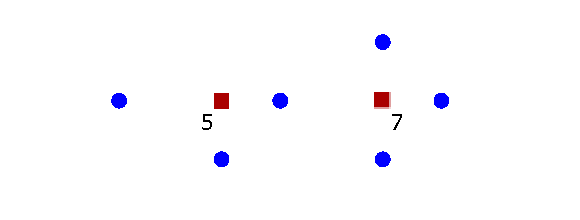
\includegraphics[scale=1.9]{imgs/fl1.pdf}\vspace{-1cm}
              \end{tcolorbox}
            \begin{tcolorbox}
              \vspace{-1cm}\hspace{-2.3cm}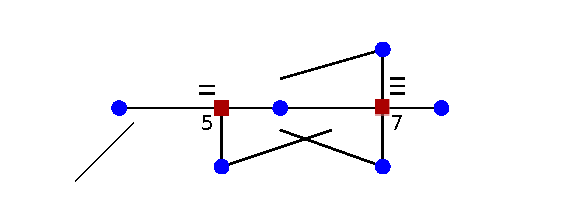
\includegraphics[scale=1.9]{imgs/fl3.pdf}\vspace{-1cm}
            \end{tcolorbox}
            
         \end{column}

         \begin{column}{0.23\paperwidth}
          \begin{tcolorbox}
            \vspace{-1cm}\hspace{-2.3cm}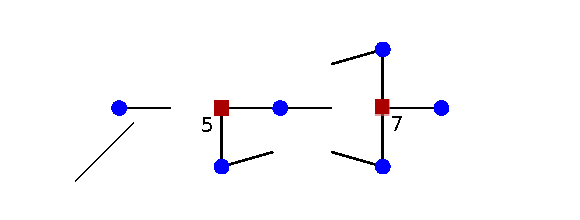
\includegraphics[scale=1.9]{imgs/fl2.pdf}\vspace{-1cm}
          \end{tcolorbox}

          \begin{tcolorbox}
            \vspace{-1cm}\hspace{-2.3cm}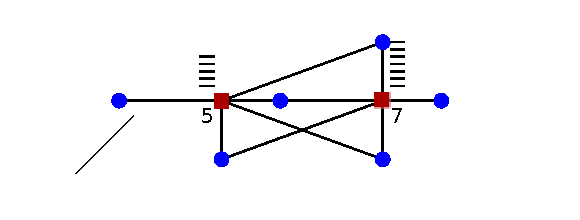
\includegraphics[scale=1.9]{imgs/fl4.pdf}\vspace{-1cm}
          \end{tcolorbox}
        \end{column}
      \end{columns}

    \end{block}

    \begin{block}{Conclusões}
      Vários algoritmos foram estudados para cada um dos três problemas. De todos esses, escolhemos um de cada problema para ser apresentado aqui. Além disso, também estudamos os melhores resultados de inaproximabilidade para cada um desses problemas.

      Além dos algoritmos apresentados, destaco também um algoritmo sofisticado para o problema das $k$-medianas métrico, desenvolvido por Li e Svensson [4]. Esse algoritmo trouxe avanço para um problema que estava há mais de uma década sem novos resultados. Eles mostraram que, para construir uma $(\alpha + \epsilon)$-aproximação para o problema das $k$-medianas métrico, é suficiente encontrar um algoritmo que devolve uma pseudo solução, ou seja, um conjunto com mais que $k$ instalações, com custo $\alpha$ vezes o ótimo. Esse resultado ampliou as possibilidades de pesquisa, evidenciando que soluções que não se limitam exatamente a $k$ instalações também podem trazer contribuições relevantes para o campo. Embora esse não seja o estado da arte para o problema das $k$-medianas métrico, os melhores resultados existentes hoje são derivados direto desse trabalho.
    \end{block}
    \begin{block}{Agradecimentos}
      O presente trabalho foi realizado com apoio da Fundação de Amparo à Pesquisa do Estado de São Paulo (FAPESP), Brasil. Processo nº 2023/16197-0.
    
      Análises desses e de outros algoritmos para esses problemas podem ser encontradas em \href{https://linux.ime.usp.br/~alvesjg/mac0499/}{https://linux.ime.usp.br/~alvesjg/mac0499}
      
    \end{block}
  \end{column}
\end{columns}

% ---------------------------------------------------------------------------- %
\end{frame}
\end{document}a